\documentclass[a4paper,12pt,draft]{article}

\usepackage[utf8]{inputenc}
\usepackage[T1]{fontenc}
\usepackage{amssymb}
\usepackage{amsmath}
\usepackage{epigraph}						% Funny quotes
\usepackage{bm}								% Bold face for vectors/matrices
\usepackage[hidelinks]{hyperref}			% Invisible, clickable links in pdf
\usepackage{listings}						% Display source code nicely
\usepackage{mcode}							% Ditto MATLAB code
\usepackage{algpseudocode}					% Nice Al Gore Rhythms
\usepackage{graphicx}						% Including graphics
\usepackage{epstopdf}						% Self-explanatory
\usepackage{float} 							% Better float placing (H option)
\usepackage{siunitx}						% SI units
\bibliographystyle{ieeetr}					% Citations in IEEE style
\lstset{frame=topbottom}

\newcommand{\M}[1]{\bm{#1}} 				% Use for variable matrices
\newcommand{\Mc}[1]{\mathbf{#1}} 			% Use for constant matrices (I, etc.)
\newcommand{\V}[1]{\mathbf{#1}} 			% Use for vectors
\newcommand{\transpose}{^{\text{T}}} 		% Make a guess, bitch
\newcommand{\sub}[1]{_{\textnormal{#1}}} 	% For upright subscripts

\lstset{
    frame=single,
    breaklines=true,
    postbreak=\raisebox{0ex}[0ex][0ex]{\ensuremath{\color{green}\hookrightarrow\space}},
    morekeywords={model, import, constant, parameter, equation, end},
    keywordstyle=\color{blue},
    numbers=left,
    numberstyle=\scriptsize,
    stepnumber=1,
    numbersep=8pt
}

\begin{document}

\begin{titlepage}
\begin{center}

\textsc{\LARGE TTK4135}\\[1.5cm]
\textsc{\LARGE Report} \linebreak
{ \huge \bfseries \textcolor[rgb]{0,0,1}{Helicopter Lab}\\[0.5cm] }
\today \vspace{1cm} \linebreak 
\emph{\textbf{Student numbers:}} \linebreak 
742434 \linebreak
XXXXXX \linebreak
XXXXXX \linebreak
XXXXXX \linebreak
XXXXXX \linebreak\linebreak \textbf{Group 9}  \vspace{3cm}\linebreak \linebreak

\textsc{Faculty of Information Technology, Mathematics and Electrical Engineering}\linebreak
\textsc{Department of Engineering Cybernetics} 
\vfill



\includegraphics[width=200pt, keepaspectratio=true]{logo_ntnu_eng.eps}

\end{center}
\end{titlepage}
\begin{abstract}

This is a report for the mandatory lab exercise in the course TTK4135 Optimization and Control held at NTNU the spring 2015. The purpose of this exercise is to get practical experience in formulating dynamic optimization problems, discretizise them and solve them using a computer, as well as using these results to impliment optimal controllers with and without feedback. The optimization problems that got solved were quadratic minimization problems, and the feedback was introduced using LQ controllers.

\end{abstract}

\tableofcontents

\section{Introduction}

This is a lab called the Helicopter Lab. As the name indicates we are going to control a model of a helicopter in different ways. The system with its hardware is described in detail in \cite{_helicopter_2015}. A model of the helicopter with regulators is allready made for us. The objective is for us, the students, to find an optimal sequence of inputs that will steer the helicopter on the desired path. This will be done by formulating optimization problems, and solving them. We will solve them as discrete problems using MATLAB, wich mean that we first have to discretize our system. This input sequense we give to our system using Simulink/QuaRC. We will run our helicopters using the optimal input directly, and them compare the behaviour when we introduce feedback.

In this report we will be presenting our results in the same order that we obtained them, meaning we will have one section for each exercise in \cite{_helicopter_2015}, where the relevant math, code, plots, results, etc. will be added. The discussion will be done consecutively, with the exeption of one summarizing discution at the end of the report. 
\section{Repetition/introduction to Simulink/QuaRC (10.1)}

The first exercise in the exercise set was meant as a repetition for those that have completed the Helicopter lab in the course TTK4115 Linear System Theory, and a introduction to Simulink/QuaRC for the rest. In our group everyone have completed the lab from TTK4115, and we didn't use much time on this problem. We ran the Simulink/QuaRC-program, and observed that premade controllers were behaving fine. We changed the setpoints in real-time, and immediately got satisfying responses from the helicopter.
\epigraph{\textit{'Smack my pitch up.'}}{The Prodigy (1997)}

\section{Optimal control of pitch/travel without feedback}

%%%%%%%%%%%%%%%%%%%%%%%%%%%%%%%%%%%%%%%%%%%%%%%%%%%%%%%%%%%%
\subsection{State space form (10.2.1)}
%%%%%%%%%%%%%%%%%%%%%%%%%%%%%%%%%%%%%%%%%%%%%%%%%%%%%%%%%%%%
We want to write the model \eqref{eq:model1} in continuous time state space form with states and input as shown in \eqref{eq:state_and_input}.

\begin{equation}\label{eq:model1}
	\V{\dot{x}} = \M{A}_{c}\V{x} + \M{B}_{c}u
\end{equation}

\begin{subequations}\label{eq:state_and_input}
\begin{align}
	\V{x} 	&= \begin{bmatrix}\lambda & r & p & \dot{p} \end{bmatrix}\transpose \\
	u 		&= p_{c}
\end{align}
\end{subequations}

The equations of motion for the states are shown in \eqref{eq:state_equations} and the constants used are defined in \eqref{eq:K1K2}.

\begin{subequations}\label{eq:state_equations}
\begin{align}
	\dot{\lambda} 	&= r \\
	\dot{r} 		&= - K_{a} p \\
	\dot{p} 		&= \dot{p} \\
	\ddot{p} 		&= K_{1} K_{pp} (p_{c} - p) - K_{1} K_{pd} \dot{p}
\end{align}
\end{subequations}

\begin{subequations}\label{eq:K1K2}
\begin{align}
	K_{1} &= \frac{K_{f} l_{n}}{J_{p}} \\
	K_{2} &= \frac{K_{p} l_{a}}{J_{t}}
\end{align}
\end{subequations}

The above gives the result in \eqref{eq:state_space_matrices}.

\begin{equation}\label{eq:state_space_matrices}
	\V{\dot{x}} =
	\underbrace{
		\begin{bmatrix}
			0 & 1 & 0 				& 0 \\
			0 & 0 & -K_{2} 			& 0 \\
			0 & 0 & 0 				& 1 \\
			0 & 0 & -K_{1}K_{pp}	& -K_{1}K_{pd}
		\end{bmatrix}
	}_{\M{A}_{c}}
	\V{x} +
	\underbrace{
		\begin{bmatrix}
			0 \\ 0 \\ 0 \\ K_{1}K_{pp}
		\end{bmatrix}
	}_{\M{B}_{c}}
	u
\end{equation}


%%%%%%%%%%%%%%%%%%%%%%%%%%%%%%%%%%%%%%%%%%%%%%%%%%%%%%%%%%%%
\subsection{Model discussion (10.2.1)}
%%%%%%%%%%%%%%%%%%%%%%%%%%%%%%%%%%%%%%%%%%%%%%%%%%%%%%%%%%%%
The states are travel, travel rate, pitch, and pitch rate. The controller output is the pitch setpoint to be used by the already implemented controller which in turn calculates voltage inputs for the plant. Thus, we are modelling not the helicopter alone, but a system that consists of the helicopter along with the given controller. This corresponds with Figure 7 (proper ref here?) in the exercise text (add ref).


%%%%%%%%%%%%%%%%%%%%%%%%%%%%%%%%%%%%%%%%%%%%%%%%%%%%%%%%%%%%
\subsection{Discretisation (10.2.2)}
%%%%%%%%%%%%%%%%%%%%%%%%%%%%%%%%%%%%%%%%%%%%%%%%%%%%%%%%%%%%
We discretise the system by the Forward Euler Method. The general definition of the method and how it relates to our system is described by equations \eqref{eq:forward_euler} and \eqref{eq:euler_func}, respectively.

\begin{equation}\label{eq:forward_euler}
	y_{k+1} = y_{k} + h f(x_{k}, y_{k})
\end{equation}

\begin{equation}\label{eq:euler_func}
	f = \left( \M{A}_{c} \V{x}_{k} + \M{B}_c u_{k} \right)
\end{equation}

Using \eqref{eq:forward_euler} and \eqref{eq:euler_func}, we can find the matrices of the discretised system, as shown in \eqref{eq:disc} and \eqref{eq:disc_matrices}.

\begin{subequations}\label{eq:disc}
\begin{align}
	\V{x}_{k+1} &= \V{x}_{k} + \left( \M{A}_{c} \V{x}_{k} + \M{B}_c u_{k} \right) h \\
				&= \V{x}_{k} + h\M{A}_{c}\V{x}_{k} + h\M{B}_{c}u_{k} \\
				&= \left( \Mc{I} + h\M{A}_{c} \right) \V{x}_{k} + h\M{B}_{c}u_{k} \\
				&= \M{A}\V{x}_{k} + \M{B}u_{k}
\end{align}
\end{subequations}

\begin{subequations}\label{eq:disc_matrices}
\begin{equation}
	\M{A} = \Mc{I} + h\M{A}_{c} =
	\begin{bmatrix}
		1 & h & 0 & 0 \\
		0 & 1 & -K_{2}h & 0 \\
		0 & 0 & 1 & h \\
		0 & 0 & -K_{1}K_{pp}h	& 1-K_{1}K_{pd}h
	\end{bmatrix}
\end{equation}
\begin{equation}
	\M{B} = h\M{B}_c =
	\begin{bmatrix} 0 \\ 0 \\ 0 \\ K_{1}K_{pp}h \end{bmatrix}
\end{equation}
\end{subequations}

%%%%%%%%%%%%%%%%%%%%%%%%%%%%%%%%%%%%%%%%%%%%%%%%%%%%%%%%%%%%
\subsection{Cost function discussion}
%%%%%%%%%%%%%%%%%%%%%%%%%%%%%%%%%%%%%%%%%%%%%%%%%%%%%%%%%%%%
- cost function has a focus on the error between $\lambda_i$ and $\lambda_f$
- is a quadratic function, least-square 

%%%%%%%%%%%%%%%%%%%%%%%%%%%%%%%%%%%%%%%%%%%%%%%%%%%%%%%%%%%%
\subsection{unwatend effect dicsussion}
%%%%%%%%%%%%%%%%%%%%%%%%%%%%%%%%%%%%%%%%%%%%%%%%%%%%%%%%%%%%
- when $\lambda = \lambda_f$, you will minimize the pitch, making it 0. This can make the helicopter oscilate around $\lambda = \lambda_f$, as the pitch will be set to 0 on that particular point

%%%%%%%%%%%%%%%%%%%%%%%%%%%%%%%%%%%%%%%%%%%%%%%%%%%%%%%%%%%%
\subsubsection{4 does the helicopter end in desired and what causes deviation}
%%%%%%%%%%%%%%%%%%%%%%%%%%%%%%%%%%%%%%%%%%%%%%%%%%%%%%%%%%%%
- No, because the optimization calculation doesn't take in account the brake time to stop in the desired point, and thus it doesn't stop in time.

\epigraph{\textit{'I've got 99 problems, but a pitch ain't one.'}}{Ice-T (1993)}

\section{Optimal control of pitch/travel with LQ control}

\section{MPC discussion}

\subsection{how would you realize MPC}
look at exercise 

\subsection{discuss advantages and disadvantages with MPC compared to the one you have implemented}
MPC: a lot of computations, heavy for the computer, slow, but very accurate
LQR: not that much computations, generally fast, not that accurate

\subsection{think about how the structure in fig 8 would look if you used MPC}
\epigraph{\textit{'A helicopter does not want to fly, it just vibrates so much that the ground rejects it.'}}{Kurt Vonnegut}

\section{Optimal control of pitch/travel and elevation with and without feedback (10.4)}

%%%%%%%%%%%%%%%%%%%%%%%%%%%%%%%%%%%%%%%%%%%%%%%%%%%%%%%%%%%%
\subsection{Discretisation with elevation states (10.4.1)} \label{10.4.1}
%%%%%%%%%%%%%%%%%%%%%%%%%%%%%%%%%%%%%%%%%%%%%%%%%%%%%%%%%%%%
We will re-formulate the continuous system \eqref{eq:system} with additional states for elevation $e$ and elevation rate $\dot{e}$. The system with new state and input vectors \eqref{eq:state_input} and state equations \eqref{eq:state_eqns} is expressed by the matrices shown in \eqref{eq:matrices}.

\begin{equation}\label{eq:system}
	\V{\dot{x}}	= \M{A} \V{x} + \M{B} \V{u}
\end{equation}

\begin{equation}\label{eq:state_input}
	\V{x} =
	\begin{bmatrix}
		\lambda & r & p & \dot{p} & e & \dot{e}
	\end{bmatrix}\transpose
	,\qquad
	\V{u} =
	\begin{bmatrix}
		p_{c} & e_{c}
	\end{bmatrix}\transpose
\end{equation}

\begin{equation}\label{eq:state_eqns}
\begin{aligned}
	\dot{\lambda}	&= r \\
	\dot{r} 		&= - K_{2} p \\
	\dot{p}			&= \dot{p} \\
	\ddot{p}		&= K_{1} K_{pp} (p_{c} - p) - K_{1} K_{pd} \dot{p} \\
	\dot{e}			&= \dot{e} \\
	\ddot{e}		&= K_{3} K_{ep} (e_{c} - e) - K_{3} K_{ed} \dot{e}
\end{aligned}
\end{equation}

\begin{equation}\label{eq:matrices}
	\V{\dot{x}} =
	\underbrace{
		\begin{bmatrix}
			0 & 1 & 0				& 0				& 0				& 0				\\
			0 & 0 & -K_{2}			& 0				& 0				& 0				\\
			0 & 0 & 0				& 1				& 0				& 0				\\
			0 & 0 & -K_{1}K_{pp}	& -K_{1}K_{pd}	& 0				& 0				\\
			0 & 0 & 0				& 0 			& 0				& 1				\\
			0 & 0 & 0				& 0				& -K_{3}K_{ep}	& -K_{3}K_{ed}	\\
		\end{bmatrix}
	}_{\M{A}_{c}}
	\V{x} +
	\underbrace{
		\begin{bmatrix}
			0			& 0				\\
			0			& 0				\\
			0			& 0				\\
			K_{1}K_{pp}	& 0				\\
			0			& 0				\\
			0			& K_{3}K_{ep}	\\
		\end{bmatrix}
	}_{\M{B}_{c}}
	\V{u}
\end{equation}

%%%%%%%%%%%%%%%%%%%%%%%%%%%%%%%%%%%%%%%%%%%%%%%%%%%%%%%%%%%%
\subsection{Discretisation again (10.4.2)}
%%%%%%%%%%%%%%%%%%%%%%%%%%%%%%%%%%%%%%%%%%%%%%%%%%%%%%%%%%%%
As in Section \ref{sec:disc1}, we again need to discretize the system. The procedure is the same; refer to the earlier Section for clarification. The result can be seen in \eqref{eq:matrix_4.2_A} and \eqref{eq:matrix_4.2_B}.

\begin{equation}
\begin{aligned}
	\V{x}_{k+1}	&= \V{x}_{k} + \left( \M{A}_{c} \V{x}_{k} + \M{B}_{c} \V{u}_{k} \right) h \\
				&= \underbrace{\left( \Mc{I} + h \M{A}_{c} \right)}_{\M{A}} \V{x}_{k}
				+ \underbrace{h \M{B}_{c}}_{\M{B}} \V{u}_{k} \\
\end{aligned}
\end{equation}

\begin{equation}\label{eq:matrix_4.2_A}
	\M{A} =
	\begin{bmatrix}
		1 & h & 0				& 0					& 0				& 0					\\
		0 & 1 & -hK_{2}			& 0					& 0				& 0					\\
		0 & 0 & 1				& h					& 0				& 0					\\
		0 & 0 & -hK_{1}K_{pp}	& 1-hK_{1}K_{pd}	& 0				& 0					\\
		0 & 0 & 0				& 0					& 1				& h					\\
		0 & 0 & 0				& 0					& -hK_{3}K_{ep}	& 1-hK_{3}K_{ed}	\\
	\end{bmatrix}
\end{equation}

\begin{equation}\label{eq:matrix_4.2_B}
	\M{B} =
	\begin{bmatrix}
		0				& 0				\\
		0				& 0				\\
		0				& 0				\\
		hK_{1}K_{pp}	& 0				\\
		0				& 0				\\
		0				& hK_{3}K_{ep}	\\
	\end{bmatrix}
\end{equation}

%%%%%%%%%%%%%%%%%%%%%%%%%%%%%%%%%%%%%%%%%%%%%%%%%%%%%%%%%%%%
\subsection{Solution of the optimization problem (10.4.3)}
%%%%%%%%%%%%%%%%%%%%%%%%%%%%%%%%%%%%%%%%%%%%%%%%%%%%%%%%%%%%

The cost function is now extended to include the elevation state, which gives us \eqref{eq:cost_function_w_elev}, with constrains given by \eqref{eq:cost_constraint_w_elev}. 

\begin{equation} \label {eq:cost_function_w_elev}
	\phi = \sum\limits_{i=1}^N (\lambda_i - \lambda_f)^2 + q_1 p_{ci}^2 + q2 e_{ci}^2
\end{equation}

\begin{equation} \label{eq:cost_constraint_w_elev}
	\alpha \exp (-\beta (\lambda_k - \lambda_t)^2) -e_k \leq 0, \quad k \in \{ 1, ..., N \}
\end{equation}

In \eqref{eq:cost_constraint_w_elev}, we used the values $\alpha = 0.2$, $\beta = 20$ and $\lambda_t = \frac{2 \pi}{3}$.
We use \texttt{fmincon} to get the result of the cost function with the constraints. The parameters used are  \texttt{vlb} and \texttt{vub}, which are vectors containing the linear constraints; \texttt{mycon}, which returns the nonlinear constraints; and \texttt{Aeq} and \texttt{beq} which are the matrices for the problem to be solved. We also send in the cost function itself and the initial values \texttt{z0}.
\begin{lstlisting}
costf = @(z) 0.5*z'*Q*z;
z = fmincon(costf, z0, [], [], Aeq, beq, vlb, vub, @mycon);
\end{lstlisting}

%%%%%%%%%%%%%%%%%%%%%%%%%%%%%%%%%%%%%%%%%%%%%%%%%%%%%%%%%%%%
\subsection{Comparison of performance with and without feedback(10.4.4)}
%%%%%%%%%%%%%%%%%%%%%%%%%%%%%%%%%%%%%%%%%%%%%%%%%%%%%%%%%%%%
Without feedback the pitch goes to 0 when $\lambda = \lambda_f$, but does not compensate to avoid overshoot. With feedback, the helicopter will change its pitch to the opposite direction, making the helicopter stop and stay still at $\lambda = \lambda_f$. 

\begin{figure}[H]
	\centering
	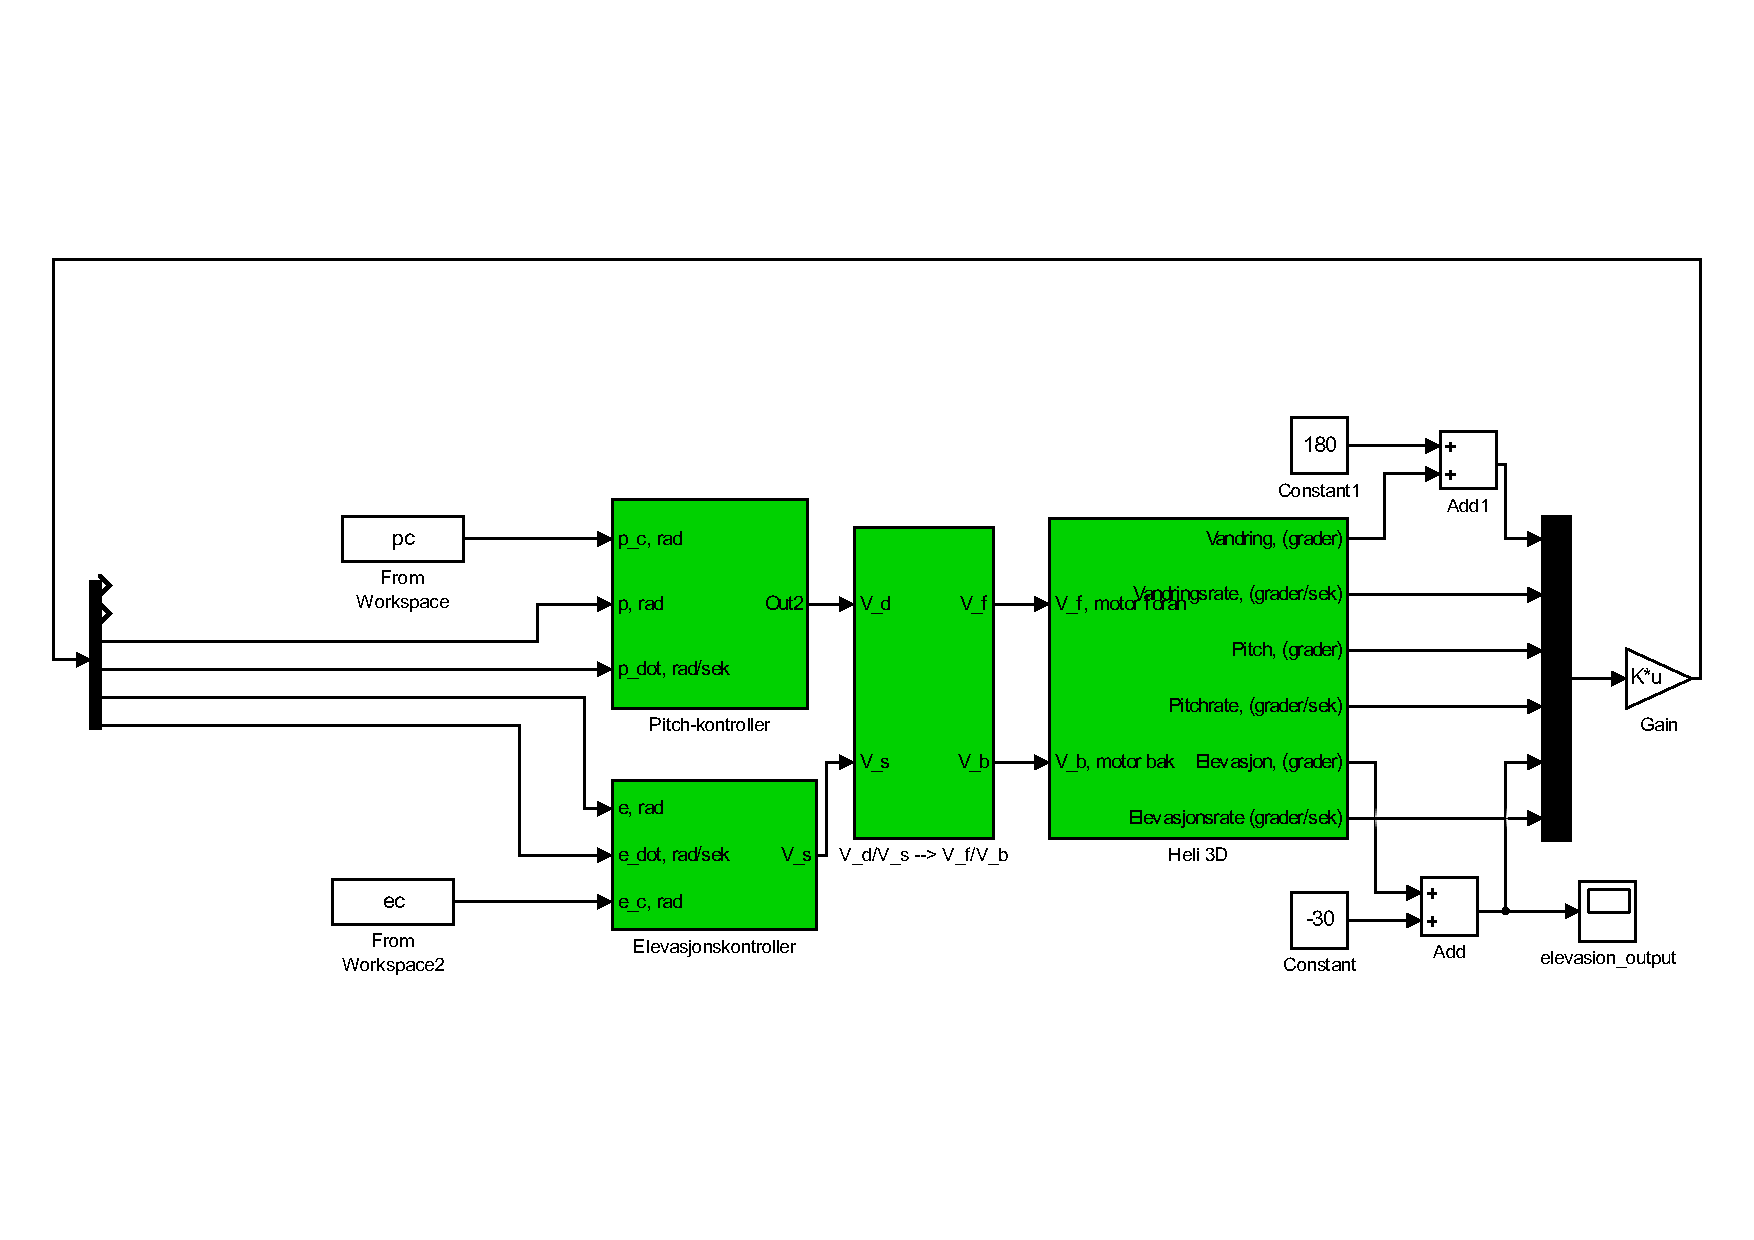
\includegraphics[width=\textwidth, trim=2cm 5cm 2cm 2cm]{simulinkmodels/heldag4UnFeed}
	\caption{Simulink model of the system without feedback}
	\label{fig:heldag4UnFeed}
\end{figure}

\begin{figure}[H]
	\centering
	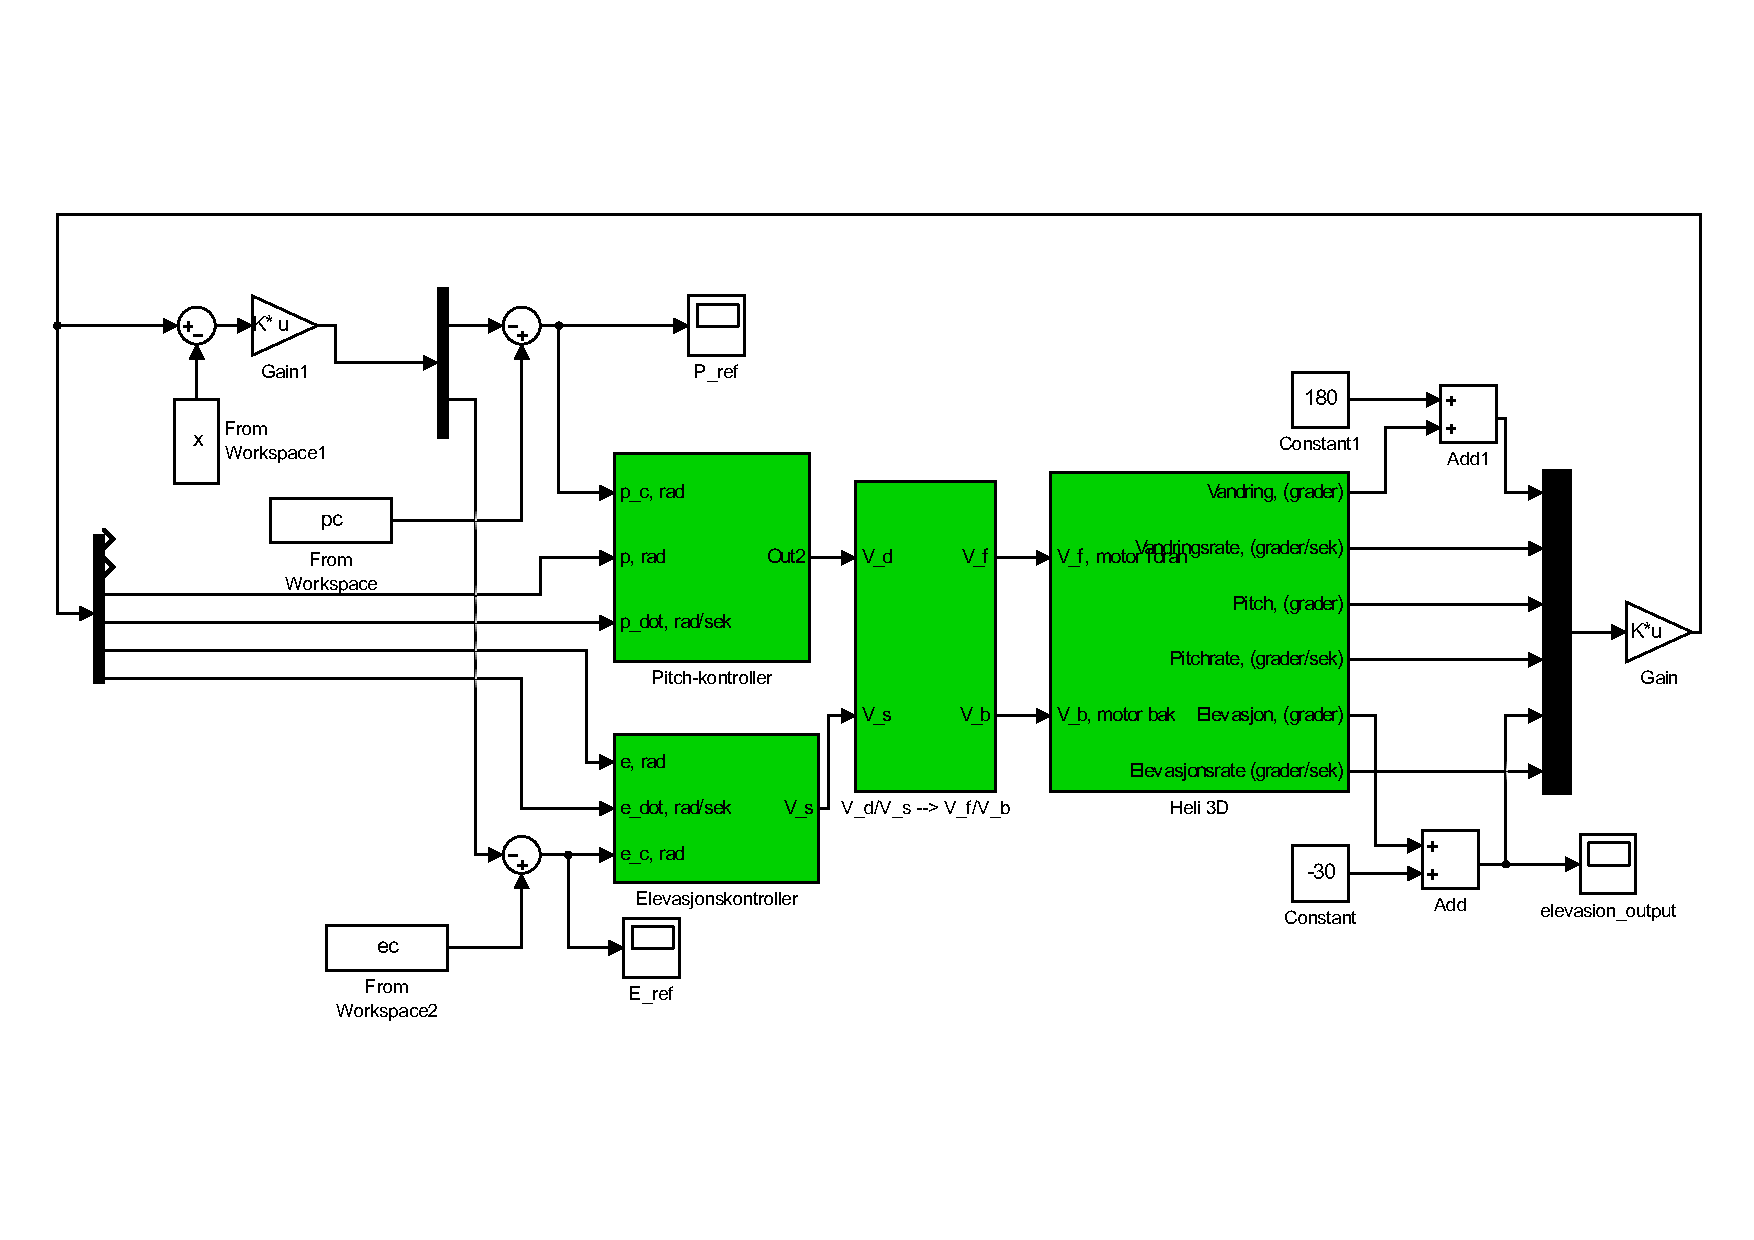
\includegraphics[width=\textwidth, trim=2cm 5cm 2cm 2cm]{simulinkmodels/heldag4medFeed}
	\caption{Simulink model of the system with feedback}
	\label{fig:heldag4medFeed}
\end{figure}

\begin{figure}[H]
	\centering
	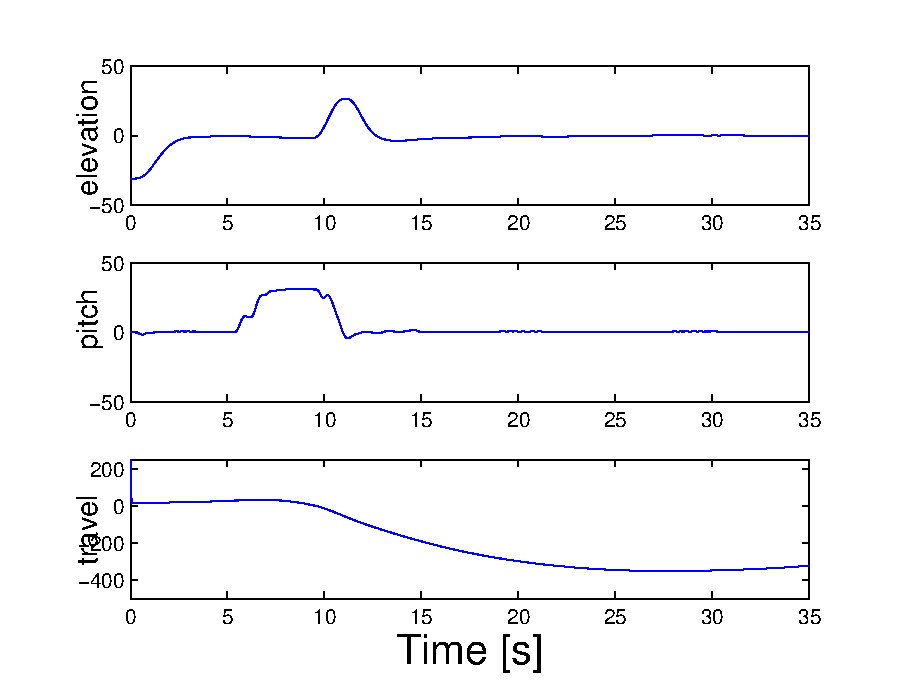
\includegraphics[width=\textwidth]{day4_nofeed}
	\caption{Actual values day 4 without feedback}
	\label{fig:day4nofeed}
\end{figure}


\begin{figure}[H]
	\centering
	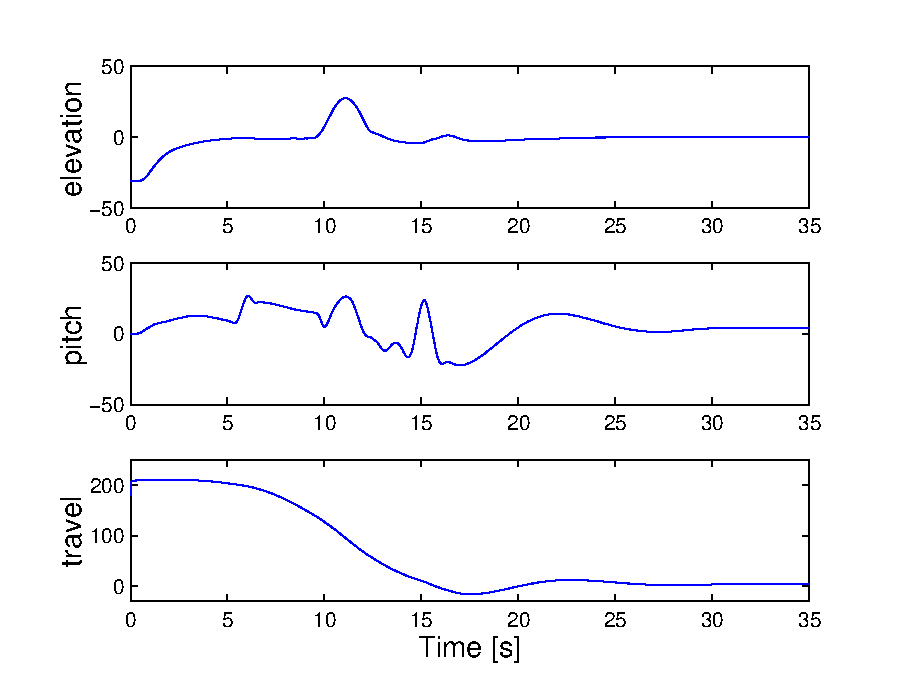
\includegraphics[width=\textwidth]{day4_yesfeed}
	\caption{Actual values day 4 with feedback}
	\label{fig:day4yesfeed}
\end{figure}

As we can see in the sensor data from the model without feedback, the helicopter does not stop at $\lambda = \lambda_f$, but keeps moving. In the model with feedback, however, it does stop at $\lambda = \lambda_f$, but the change in pitch to keep it still in the reference point also makes the helicopter elevate a bit, as can be seen in the plot at roughly 16 seconds. It also overshoots slightly, but converges at the setpoint.

In the calculated outputs you can see that it also expects some change in the pitch when trying to stop at the reference point, but it is much more subtle than the real behaviour, especially with feedback. This would correspond better if the LQR was tuned better. In the measured values of the model without feedback, this is more similar to the calculated pitch, but the travel is a bit off, as the helicopter keeps gliding after it reaches the reference point. This is improved in the model with feedback, although it does not stop as quickly and smoothly as the calculated output would suggest.

%%%%%%%%%%%%%%%%%%%%%%%%%%%%%%%%%%%%%%%%%%%%%%%%%%%%%%%%%%%%
\subsection{Discussion of decoupled states (10.4.5)}
%%%%%%%%%%%%%%%%%%%%%%%%%%%%%%%%%%%%%%%%%%%%%%%%%%%%%%%%%%%%
In real life the pitch and pitch rate of the helicopter would have an effect on both the elevation rate and the elevation itself. This will result in an offset from the calculated optimal trajectory.  
By modelling the system with the elevation and travel coupled with the pitch, you will remove the offset at the cost of a more complex model.
\section{Discussion}
The purpose of this lab was to formulate a dynamic optimization problem, and solve this using MATLAB and Simulink, as well as seeing the results of control both with and without feedback.

First, this was done by using model-based optimization to provide the pitch and elevation controllers with an input $u$, before the model was improved by adding an LQR-control layer between the optimization layer and the basic control layer. 


\section{Conclusion}
We feel that it has been interesting to work on this lab, and that we have learnt a lot by doing it. Through a practical approach to implementing optimization algorithms, we have gained insight into how it might be to work as a control system engineer and some of the problems they encounter. 
We have also seen that using optimization algorithms when making a control system makes the system more precise, and is worth both the time and energy it takes to implement them. 

All in all we think this has been a successful exercise, and it has been both rewarding and educational.
\section{Appendix}
\subsection{Variables}
\begin{center}
\begin{tabular}{l l l l}
\hline 
Symbol & Variable \\ \hline
$p$ & Pitch \\
$p_c$ & Pitch setpoint \\
$\lambda$ & Travel \\
$r$ & Travel rate \\
$r_c$ & Travel rate setpoint \\
$e$ & Elevation \\
$e_c$ & Elevation setpoint \\
$V_f$ & Voltage, front motor \\
$V_b$ & Voltage, rear motor \\
$V_d$ & Voltage difference, $V_f -V_b$ \\
$V_s$ & Voltage sum, $V_f + V_b$ \\
$K_{pp}$, $K_{pd}$, $K_{ep}$, $K_{ei}$, $K_{ed}$ & Controller gains \\
$T_g$ & Moment required to keep the helicopter flying
\end{tabular}
\end{center}
\label{table:variables}



\vspace{1cm}

\subsection{Constants}
\begin{center}
\begin{tabular}{l l l l}
\hline
Symbol & Parameter & Value & Unit \\ \hline
$l_a$ & Distance from elevation axis to helicopter body & 0.64 & m \\
$l_h$ & Distance from pitch axis to motor & 0.177 & m \\
$K_f$ & Distance from elevation axis to helicopter body & 0.1983 &\si{\newton \per \meter}  \\
$J_e$ & Moment of inertia (elevation axis) & 1.0625 & \si{\kilogram \meter \squared}  \\
$J_t$ & Moment of inertia (travel axis) & 1.0625 & \si{\kilogram \meter \squared}  \\
$J_p$ & Moment of inertia (pitch axis) & 0.0406 & \si{\kilogram \meter \squared}  \\
$m_h$ & Mass of helicopter & 1.297 &\si{\kilogram}  \\
$m_w$ & Counterweight & 1.802 & \si{\kilogram} \\
$m_g$ & Effective mass of the helicopter & 0.026 & \si{\kilogram} \\
$K_p$ & Force to lift the helicopter from the ground & 0.2551 & \si{\newton}
\end{tabular}
\end{center}
\label{table:constants}

\subsection{Code for (10.2) and (10.3)}

This code is modified from the code handed out on itslearning.

\begin{lstlisting}
init04;
delta_t	  = 0.25;	                    % sampling time
sek_forst = 5;

q = 0.1;
% System model. x=[lambda r p p_dot]'

A1 = [1 delta_t 0 0;
      0 1 -K_2*delta_t 0;
      0 0 1 delta_t;
      0 0 -K_1*K_pp*delta_t 1-K_1*K_pd*delta_t];
  
B1 = [0; 0; 0; K_1*K_pp*delta_t];

% Number of states and inputs

mx = size(A1,2);                        % Number of states (number of columns in A)
mu = size(B1,2);                        % Number of inputs(number of columns in B)

% Initial values

x1_0 = pi;                              % Lambda
x2_0 = 0;                               % r
x3_0 = 0;                               % p
x4_0 = 0;                               % p_dot
x0   = [x1_0 x2_0 x3_0 x4_0]';          % Initial values

% Time horizon and initialization

N  = 100;                                % Time horizon for states
M  = N;                                 % Time horizon for inputs
z  = zeros(N*mx+M*mu,1);                % Initialize z for the whole horizon
z0 = z;                                 % Initial value for optimization

% Bounds

ul 	    = -30*pi/180;                   % Lower bound on control -- u1
uu 	    = 30*pi/180;                    % Upper bound on control -- u1

xl      = -Inf*ones(mx,1);              % Lower bound on states (no bound)
xu      = Inf*ones(mx,1);               % Upper bound on states (no bound)
xl(3)   = ul;                           % Lower bound on state x3
xu(3)   = uu;                           % Upper bound on state x3

% Generate constraints on measurements and inputs

[vlb,vub]       = genBegr2(N,M,xl,xu,ul,uu);
vlb(N*mx+M*mu)  = 0;                    % We want the last input to be zero
vub(N*mx+M*mu)  = 0;                    % We want the last input to be zero

% Generate the matrix Q and the vector c (objecitve function weights in the QP problem) 

Q1 = zeros(mx,mx);
Q1(1,1) = 1;                            % Weight on state x1
Q1(2,2) = 0;                            % Weight on state x2
Q1(3,3) = q;                            % Weight on state x3
Q1(4,4) = 0;                            % Weight on state x4
P1 = q;                                 % Weight on input
Q = 2*genq2(Q1,P1,N,M,mu);              % Generate Q
c = zeros(N*mx+M*mu,1);                 % Generate c

% Generate system matrixes for linear model

Aeq = gena2(A1,B1,N,mx,mu);          % Generate A
beq = zeros(1, size(Aeq,1));         % Generate b
beq(1:mx) = A1*x0; 	        	        % Initial value

% Solve Qp problem with linear model
tic
[z,lambda] = quadprog(Q, c, [], [], Aeq, beq, vlb, vub, z0);
t1=toc;


% Extract control inputs and states

u  = [z(N*mx+1:N*mx+M*mu);z(N*mx+M*mu)]; % Control input from solution

x1 = [x0(1);z(1:mx:N*mx)];              % State x1 from solution
x2 = [x0(2);z(2:mx:N*mx)];              % State x2 from solution
x3 = [x0(3);z(3:mx:N*mx)];              % State x3 from solution
x4 = [x0(4);z(4:mx:N*mx)];              % State x4 from solution

Antall = 5/delta_t;
Nuller = zeros(Antall,1);
Enere  = ones(Antall,1);

u   = [Nuller; u; Nuller];
x1  = [pi*Enere; x1; Nuller];
x2  = [Nuller; x2; Nuller];
x3  = [Nuller; x3; Nuller];
x4  = [Nuller; x4; Nuller];

%save trajektor1ny
t = 0:delta_t:delta_t*(length(u)-1); % real time

simin = [t' u];

% figure
                

figure(2)
subplot(511)
stairs(t,u),grid
ylabel('u')
subplot(512)
plot(t,x1,'m',t,x1,'mo'),grid
ylabel('lambda')
subplot(513)
plot(t,x2,'m',t,x2','mo'),grid
ylabel('r')
subplot(514)
plot(t,x3,'m',t,x3,'mo'),grid
ylabel('p')
subplot(515)
plot(t,x4,'m',t,x4','mo'),grid
xlabel('tid (s)'),ylabel('pdot')

x = [t' x1 x2 x3 x4];
%%

Q_k = [25 0 0 0;
       0 0.5 0 0;
       0 0 100 0;
       0 0 0 0.5];
R = 1;

[K S E] = dlqr(A1, B1, Q_k, R, 0);

\end{lstlisting}

\subsection{Code for (10.4)}

This code is modified from the code handed out on itslearning.

\begin{lstlisting}
init04;
delta_t	  = 0.25;	                    % sampling time
sek_forst = 5;

q = 0.1;
% System model. x=[lambda r p p_dot]'

A = [1 delta_t 0 0 0 0;
      0 1 -K_2*delta_t 0 0 0;
      0 0 1 delta_t 0 0;
      0 0 -K_1*K_pp*delta_t 1-K_1*K_pd*delta_t 0 0;
      0 0 0 0 1 delta_t;
      0 0 0 0 -delta_t*K_3*K_ep 1-delta_t*K_3*K_ed];
  
B = [0 0; 0 0; 0 0; K_1*K_pp*delta_t 0; 0 0; 0 delta_t*K_3*K_ep];

% Number of states and inputs

mx = size(A,2);                        % Number of states (number of columns in A)
mu = size(B,2);                        % Number of inputs(number of columns in B)

% Initial values

x1_0 = pi;                              % Lambda
x2_0 = 0;                               % r
x3_0 = 0;                               % p
x4_0 = 0;                               % p_dot
x5_0 = 0;                               % e
x6_0 = 0;                               % e_dot
x0   = [x1_0 x2_0 x3_0 x4_0 x5_0 x6_0]';          % Initial values

u1_0 = 0;
u2_0 = 0; % ask studass

q_1 = 1;
q_2 = 1;
alfa = 0.2;
beta = 20;
lambda_t = 2*pi/3;

% Time horizon and initialization

N  = 40;                                % Time horizon for states
M  = N;                                 % Time horizon for inputs
z  = zeros(N*mx+M*mu,1);                % Initialize z for the whole horizon
z0 = z;                                 % Initial value for optimization


% Bounds

ul 	    = -30*pi/180;                   % Lower bound on control -- u1
uu 	    = 30*pi/180;                    % Upper bound on control -- u1

xl      = -Inf*ones(mx,1);              % Lower bound on states (no bound)
xu      = Inf*ones(mx,1);               % Upper bound on states (no bound)
xl(3)   = ul;                           % Lower bound on state x3
xu(3)   = uu;                           % Upper bound on state x3

% Generate constraints on measurements and inputs

[vlb,vub]       = genBegr2(N,M,xl,xu,ul,uu);
vlb(N*mx+M*mu)  = 0;                    % We want the last input to be zero
vub(N*mx+M*mu)  = 0;                    % We want the last input to be zero

% Generate system matrixes for linear model
Aeq = gena2(A,B,N,mx,mu);          % Generate A
beq = zeros(1, size(Aeq,1));         % Generate b
beq(1:mx) = A*x0; 	        	        % Initial value

% Generate the matrix Q and the vector c (objecitve function weights in the QP problem) 

Q1 = zeros(mx,mx);
Q1(1,1) = 1;                            % Weight on state x1
Q1(2,2) = 0;                            % Weight on state x2
Q1(3,3) = q;                            % Weight on state x3
Q1(4,4) = 0;                            % Weight on state x4
Q1(5,5) = 0;
Q1(6,6) = 0;
P1 = zeros(mu, mu);
P1(1,1) = q_1;                            % Weight on input
P1(2,2) = q_2;
Q = 2*genq2(Q1,P1,N,M,mu);              % Generate Q
c = zeros(N*mx+M*mu,1);                 % Generate c

% Solve Qp problem with linear model

costf = @(z) 0.5*z'*Q*z;
%tic
%[z,lambda] = quadprog(Q, c, [], [], Aeq, beq, vlb, vub, z0);
%t1=toc;
nonlcon = @(z) alfa*exp(-beta*(z(1+mx)-lambda_t)^2)-z(5+mx);
z = fmincon(costf, z0, [], [], Aeq, beq, vlb, vub, @mycon);
% Calculate objective value

phi1 = 0.0;
PhiOut = zeros(N*mx+M*mu,1);
for i=1:N*mx+M*mu
  phi1=phi1+Q(i,i)*z(i)*z(i);
  PhiOut(i) = phi1;
end

% Extract control inputs and states

u1 = [u1_0; z(N*mx+1:mu:N*mx+M*mu)]; % Control input from solution
u2 = [u2_0; z(N*mx+2:mu:N*mx+M*mu)];

x1 = [x0(1);z(1:mx:N*mx)];              % State x1 from solution
x2 = [x0(2);z(2:mx:N*mx)];              % State x2 from solution
x3 = [x0(3);z(3:mx:N*mx)];              % State x3 from solution
x4 = [x0(4);z(4:mx:N*mx)];              % State x4 from solution
x5 = [x0(5);z(5:mx:N*mx)];
x6 = [x0(6);z(6:mx:N*mx)];

Antall = 5/delta_t;
Nuller = zeros(Antall,1);
Enere  = ones(Antall,1);

u1   = [Nuller; u1; Nuller];
u2   = [Nuller; u2; Nuller];

x1  = [x1_0*Enere; x1; Nuller];
x2  = [Nuller; x2; Nuller];
x3  = [Nuller; x3; Nuller];
x4  = [Nuller; x4; Nuller];
x5 = [Nuller; x5; Nuller];
x6 = [Nuller; x6; Nuller];

%save trajektor1ny
t = 0:delta_t:delta_t*(length(u1)-1); % real time

pc = [t' u1];
ec = [t' u2];
% figure
                

figure(2)
subplot(8,1,1)
stairs(t,u1),grid
ylabel('u1')
subplot(8,1,2)
stairs(t, u2),grid
ylabel('u2')
subplot(8,1,3)
plot(t,x1,'m',t,x1,'mo'),grid
ylabel('lambda')
subplot(8,1,4)
plot(t,x2,'m',t,x2','mo'),grid
ylabel('r')
subplot(8,1,5)
plot(t,x3,'m',t,x3,'mo'),grid
ylabel('p')
subplot(8,1,6)
plot(t,x4,'m',t,x4','mo'),grid
ylabel('pdot')
subplot(8,1,7)
plot(t,x5,'m',t,x5','mo'),grid
ylabel('e')
subplot(8,1,8)
plot(t,x6,'m',t,x6','mo'),grid
ylabel('edot')
xlabel('tid (s)')

x = [t' x1 x2 x3 x4 x5 x6];

%%
Q_k = [2 0 0 0 0 0;
       0 1 0 0 0 0;
       0 0 1 0 0 0;
       0 0 0 1.2 0 0;
       0 0 0 0 1 0;
       0 0 0 0 0 1.5];

R = [1 0;
     0 1];

[K S E] = dlqr(A, B, Q_k, R, 0);

\end{lstlisting}
%\section{Pastebin (remove before handing in lol)}

%%%%%%%%%%%%%%%%%%%%%%%%%%%%%%%%%%%%%%%%%%%%%%%%%%%%%%%%%%%%
\subsection{Bibtex test}
%%%%%%%%%%%%%%%%%%%%%%%%%%%%%%%%%%%%%%%%%%%%%%%%%%%%%%%%%%%%
\cite{nocedal_numerical_2006} and \cite{_helicopter_2015} are pretty cool.

%%%%%%%%%%%%%%%%%%%%%%%%%%%%%%%%%%%%%%%%%%%%%%%%%%%%%%%%%%%%
\subsection{mcode test}
%%%%%%%%%%%%%%%%%%%%%%%%%%%%%%%%%%%%%%%%%%%%%%%%%%%%%%%%%%%%
\lstinputlisting[label={lst:dog}, caption={A dog.}]{blkdiag.m}

\begin{figure}[H]
	\centering
	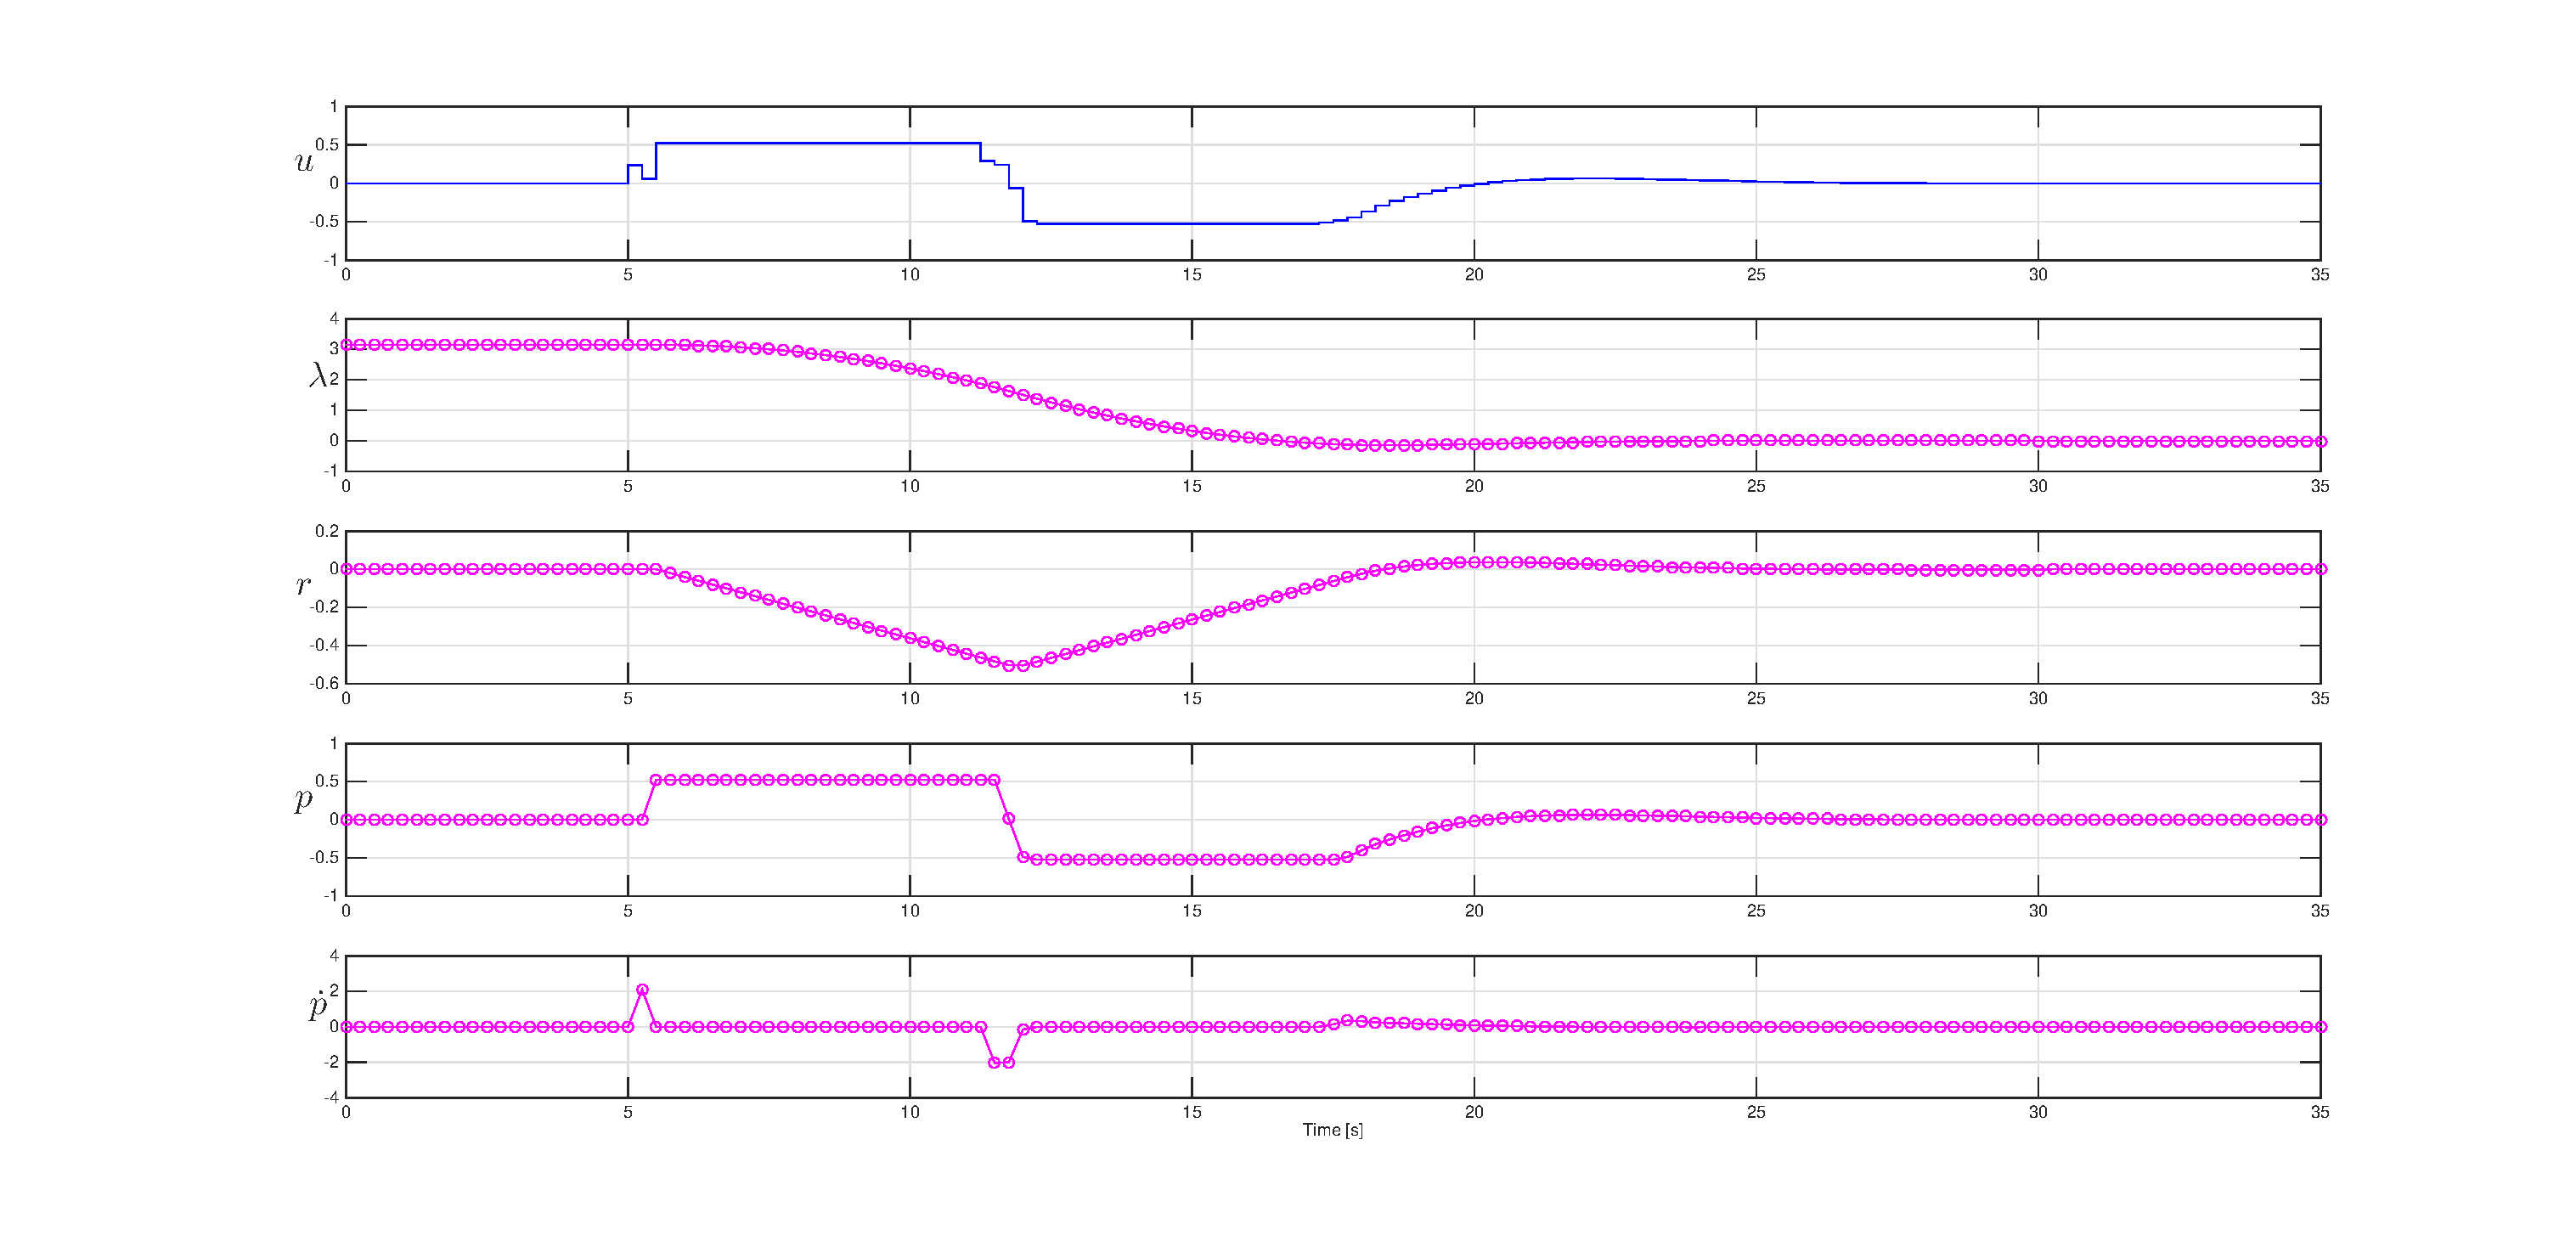
\includegraphics[width=\textwidth]{Opp10_3-good}
	\caption{Digraph.}
	\label{fig:digraph}
\end{figure}


\bibliography{ref-helikopter}

\end{document}
